\section{Introduction}

\subsection{Balanced \textit{k}-Mean}
	\begin{frame}{Balanced \textit{k}-Means} % FIXME: reorder 3 elements`
		\begin{minipage}{0.5\textwidth} % FIXME: padding
			\textbf{Advantages over classical approaches}
			\begin{itemize}
				\item[$\bullet$] Better targets the global solution of the training problem  
				\item[$\bullet$] Better theoretic scalability on large datasets
			\end{itemize}
		\end{minipage}\hfill
		\begin{minipage}{0.5\textwidth}
			\textbf{Outline}
			\begin{itemize}
				\item[$\bullet$] QUBO formulation and theoretical analysis
				\item[$\bullet$] Empirical Analysis 
				\item[$\bullet$] Conclusions and considerations
			\end{itemize}
		\end{minipage}\hfill
		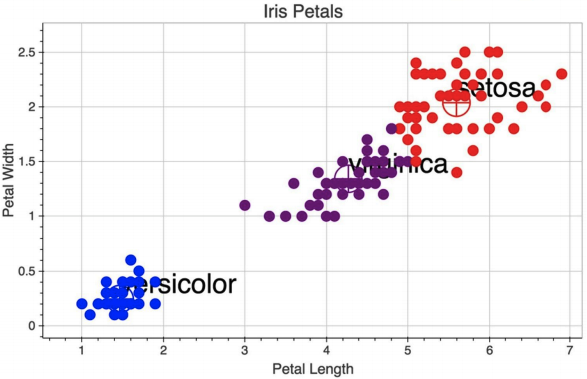
\includegraphics[width=4.3cm]{Iris.png}
	\end{frame}
	% NOTES: We want to cluster data in balanced sets, similarity is 
	% measured by statistical variance withing each cluster
	
	% The advantages ove classical approaches are…
	% This is the outline of the paper of presentation that resembles the one of the paper


\subsection{Unconstrained \textit{k}-Mean Clustering}
	\begin{frame}{Unconstrained \textit{k}-Mean Clustering}
		\textbf{Lloyd’s algorithm}
		\begin{itemize}
			\item[$\bullet$] Complexity $O(Nkdi)$ \textcolor{gray}{[13]}
			\begin{itemize}
				\item[$\circ$] $N$ number of data points
				\item[$\circ$] $k$ number of clusters 
				\item[$\circ$] $d$ dimension of the dataset
				\item[$\circ$] $i$ number of iterations before the algorithm converges
			\end{itemize} 
		\end{itemize}
		\textbf{Scikit-learn implementation}
		\begin{itemize}
			\item[$\bullet$] Complexity $O(Nkd)$ \textcolor{gray}{[18]}
		\end{itemize}
		\tiny{ % FIXME: attach to bottom
			\textcolor{gray}{
				\begin{minipage}{0.5\textwidth} % FIXME: padding
					[13] J. A. Hartigan and M. A. Wong, “Algorithm AS 136: A K-Means clustering algorithm” Applied Statistics
				\end{minipage}\hfill
				\begin{minipage}{0.5\textwidth} 
					[18]“Scikit-learn: Machine learning in python,” J. Mach. Learn. Res.
				\end{minipage}\hfill
			}
		}
	\end{frame}
	

	% Lloyd’s algorithm is an iterative approach for solving unconstrained 
	% k-means clustering (meaning that the result is not necessarily balanced). 
	% The complexity is….

	% The authors use the Scikit-learn implementation (which bounds the number of iterations) as a point of comparison.
	


\section{QUBO Formulation}